\setcounter{figure}{0}
\setcounter{table}{0}
\setcounter{equation}{0}

\irsection{Input Control File and Using \Rocburn}{Input}

Two example versions of the \Rocburn\ input file (\irfilename{RocburnPYControl.txt}) are shown below. The first is a table that groups the input parameters by similarity as well as provides other information, such as the variable mapping between the theory (\irref{Section}{Theory}) and the program (\irref{Section}{Code}). The second version shows a real, working \Rocburn\ problem for the NAWC \#13 motor. In either version, note that some parameters refer to the solid (condensed) phase and some to the gas phase.

\newpage

\irssection{Summary of Input Parameters}{Summary}

\begin{small}
\begin{center}
\textbf{Annotated \Rocburn\ Input (Control) Parameters}
\end{center}

Note: The parameters given below have been rearranged by group according to similarity. This format \textbf{\underline{cannot}} be used with as an actual \Rocburn\ input file because the code requires a specific ordering. A working \Rocburn\ problem is given in \irref{Section}{Control}.

\begin{center}
\begingroup
\setlength{\LTleft}{-0.5in plus -1fill}
\setlength{\LTright}{\LTleft}
\begin{longtable}[H]{ m{2.2cm} | m{1.0cm} m{1.5cm} | m{5.5cm} | m{1.9cm} | m{2.7cm} m{1.2cm} }
\hline
\hline
	\multicolumn{1}{c}{\textbf{Input}} &
	\multicolumn{2}{c}{\textbf{Usage}} &
	\multicolumn{1}{c}{\textbf{Description}} &
	\multicolumn{1}{c}{\textbf{Units}} &
	\multicolumn{2}{c}{\textbf{Range (Typical)}} \\ \hline
\endfirsthead

\multicolumn{7}{r}{\textit{\footnotesize $\ldots$continued from last page}} \\
\hline
	\multicolumn{1}{c}{\textbf{Input}} &
	\multicolumn{2}{c}{\textbf{Usage}} &
	\multicolumn{1}{c}{\textbf{Description}} &
	\multicolumn{1}{c}{\textbf{Units}} &
	\multicolumn{2}{c}{\textbf{Range (Typical)}} \\ \hline
\endhead

\hline \multicolumn{7}{r}{\textit{\footnotesize continued on next page$\ldots$}} \\
\endfoot

\endlastfoot

\hline \multicolumn{7}{c}{\textcolor{RoyalBlue}{\textit{\textbf{Empirical burning rate (power law) model parameters}}}} \\ \hline \hline
\texttt{a\_p} & $A_p$ & \ireq{eq}{eq:pyro1} & steady state regression speed at reference pressure & cm/s & $A_p>0$ & (0.4) \\ \hline

\texttt{n\_p} & $n_p$ & \ireq{eq}{eq:pyro1} & pressure exponent & none & $0-10$ & (0.5) \\ \hline

\texttt{Pref} & $P_{\rm ref}$ & \ireq{eq}{eq:pyro1} & reference pressure & atm & $0-200$ & (35) \\ \hline 

\hline \multicolumn{7}{c}{\textcolor{RoyalBlue}{\textit{\textbf{Combustion (pyrolysis) model parameters}}}} \\ \hline \hline

\texttt{Ac} & $A_c$ & \ireq{eq}{eq:pyro2} & pre-exponential factor & cm/s & $A_c > 100$ & (2e5) \\ \hline

\texttt{eg\_ru} & $E_g/R_u$ & \ireq{eq}{eq:tstar} & scaled activation energy for gas phase (i.e., gas temperature) & K & $E_g/R_u > 100$ & (2.5e4) \\ \hline

\texttt{ec\_ru} & $E_c/R_u$ & \ireq{eqs}{eq:pyro2} & scaled activation energy for solid phase (i.e., solid temperature) & K & $E_c/R_u > 100$ & (1.3e4) \\ \hline

\texttt{alfac} & $\alpha_c$ & \ireq{eq}{eq:gofT} & condensed phase thermal diffusivity & $\SIper{}{\square\centi\meter\per\second}$ & $0-1$ & (2e-3) \\ \hline

\texttt{C} & $c_p$ & \ireq{eq}{eq:sld} & specific heat of the solid & $\SIper{}{\calorie\per\gram\per\kelvin}$ & $0-1$ & (0.4) \\ \hline

\texttt{lamg} & $\lambda_g$ & \ireq{eq}{eq:hfilmcoefffull} & gas phase thermal conductivity & $\SIper{}{\calorie\per\centi\meter\per\second\per\kelvin}$ & $0-1$ & (2e-4) \\ \hline

\texttt{delt} & $\Delta t$ & \ireq{eq}{eq:fotimeint} & simulation timestep & s & none & (3e-6) \\ \hline

\texttt{Tstar0} & $T_\star^0$ & \ireq{eq}{eq:tstar} & steady state (adiabatic) flame temperature & K & $T_{\rm ignition}-10,000$ & (2500) \\ \hline

\texttt{To} & $T_\infty$ & \ireq{eq}{eq:gofT} & supply (ambient) temperature & K & $100-1000$ & (298) \\ \hline

\hline \multicolumn{7}{c}{\textcolor{RoyalBlue}{\textit{\textbf{Ignition model parameters}}}} \\ \hline \hline

\texttt{Tignition} & none & none & ignition temperature  & K  & $T_{\rm ignition} > T_\infty$ & (850) \\ \hline

\texttt{Tsurf} & none & none & surface temperature & K & $100-T_\star^0$ & (300) \\ \hline

\texttt{film\_cons} & $h/\lambda_c$ & \ireq{eq}{eq:qc} & film constant to determine heat flux in non-burning cells & $\SIper{}{\watt\per\square\meter\per\kelvin}$ & none & (550) \\ \hline

\texttt{ixsymm} & none & none & enable/disable (axisymmetric) burning in cells at $t = 0$ & none & $0-3$ & (0) \\ \hline

\texttt{x\_surf\_burn} & none & none & width of propellant burning at $t = 0$ & m & none & (0.2) \\ \hline

\hline \multicolumn{7}{c}{\textcolor{RoyalBlue}{\textit{\textbf{Ranges for pressure, temperature, and burn speed (divergence boundaries)}}}} \\ \hline \hline

\texttt{press\_min} & none & none & minimum pressure allowed & Pa & none & (1e3) \\ \hline

\texttt{press\_max} & none & none & maximum pressure allowed & Pa & none & (1e8) \\ \hline

\texttt{Tf\_min} & none & none & minimum \texttt{Tflame} temperature allowed, where $T_{\rm flame}$ is the temperature of injected gas ($T_\star$) & K & none & (290) \\ \hline

\texttt{Tf\_max} & none & none & maximum \texttt{Tflame} temperature allowed, where $T_{\rm flame}$ is the temperature of injected gas ($T_\star$) & K & none & (1e4) \\ \hline

\texttt{rb\_min} & none & none & minimum burn rate allowed & $\SIper{}{\meter\per\second}$ & none & (-1e-9) \\ \hline

\texttt{rb\_max} & none & none & maximum burn rate allowed & $\SIper{}{\meter\per\second}$ & none & (1e2) \\ \hline

\hline \multicolumn{7}{c}{\textcolor{RoyalBlue}{\textit{\textbf{Grid parameters}}}} \\ \hline \hline

\texttt{igrid} & none & none & flag to specify computational grid type & none & none & (2) \\ \hline

\texttt{xmax} & none & none & width into propellant depth of interface region & m & $x_{\rm max} < 0$ & (-0.2) \\ \hline

\texttt{numx} & none & none & maximum number of $x_{\rm max}$ grid points & none & none & (100) \\ \hline

\texttt{beta} & none & none &  grid stretch constant used to resolve heat flux at surface & none & none & (1.01) \\ \hline

\hline \multicolumn{7}{c}{\textcolor{RoyalBlue}{\textit{\textbf{Enable lookup table to compute the flux $g$}}}} \\ \hline \hline

\texttt{TABUSE} & none & none &  enable/disable lookup table & none & none & (0) \\ \hline

\texttt{TABNAM} & none & none &  name of the file with table & none & none & (none) \\

\hline\hline\hline
\end{longtable}
\endgroup
\end{center}
\end{small}

As shown above, the list of required input parameters is extensive, 29 in total. Some of them are straightforward, especially the burn parameters that can be taken from literature values. There are others, however, that require more in depth discussion.

\irsssection{Combustion Model Parameters}{IgnitModel}

While the combustion model is well-documented, selecting an appropriate timestep, \texttt{delt}, is less so. Since a first-order integrator is used (\irref{Section}{NumSol}), the timestep must be small, so the integrator can be fast. As a result it is important to watch the numerical stability associated the selected timestep.

\irsssection{Ignition Model Parameters}{IgnitModel}

The ignition model in \Rocburn\ can be confusing, since a number of the parameters have similar names and are not necessarily specifically addressed by the theory presented in \irref{Section}{Theory}. For this reason, a simple schematic of a ``standard rocket'' is given in \irref{Figure}{fig:rocket} to aid in the presentation.

\begin{figure}[ht]
\centering
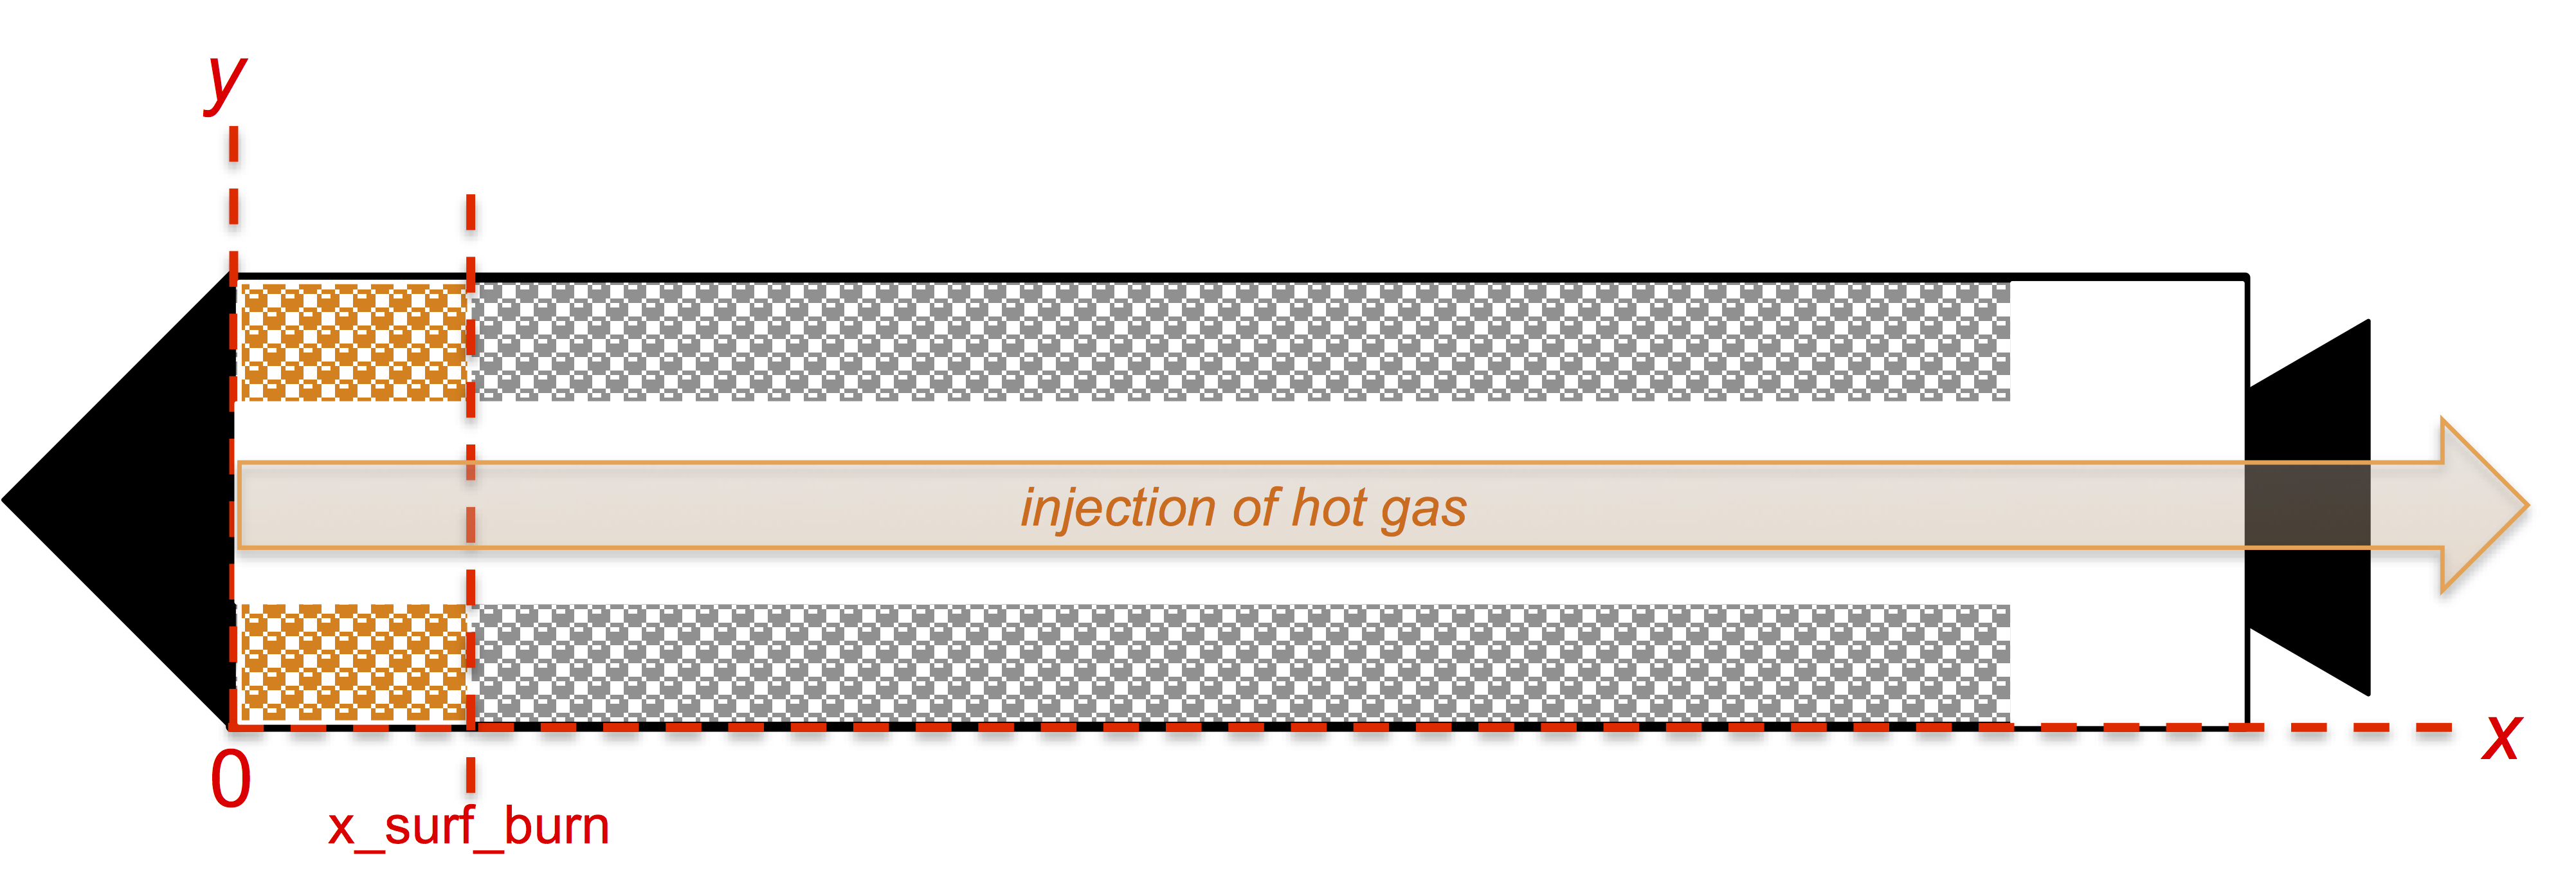
\includegraphics[width=0.9\textwidth]{../Figures/rocket.png}
\caption{Simple rocket. This schematic of a ``rocket'' illustrates the different regions, from the nozzle (far left), to the propellant (center), to the tail (far right). The variable \texttt{x\_surf\_burn} distinguishes between burning and non-burning propellant.}
\label{fig:rocket}
\end{figure}

\irref{Figure}{fig:rocket} shows a simple rocket with the nozzle at one end (left), the tail at the other (right), and the propellant in the middle. In the center of the chamber is a bore through which the gas escapes as the rocket (propellant) burns away. Depending on the situation, the propellant may or may not be burning at $t=0$ (orange vs gray propellant, respectively), and \texttt{x\_surf\_burn} (i.e., the value of $x$ that represents the burning surface) distinguishes between burning and non-burning propellant.

\irparanonum{film\_cons}{paramh} The input parameter \texttt{film\_cons} is somewhat misleading as it sounds like the film {\it coefficient}, $h$, such as in \irref{Section}{PreIgnit}. In actuality it is a combination of two constants.

\begin{equation}
{\cal C_{\rm film}} = \frac{h}{\lambda_c} = \frac{0.0287\rho_g U_\infty c_p}{\lambda_c}\left(x\rho_g U_\infty\mu_g c_p^2\over \lambda_g^2\right)^{-1/5}
\end{equation}

where $\lambda_c$ is the thermal conductivity of the solid. (See \ireq{eq}{eq:hfilmcoefffull}.) As illustrated in \irref{Section}{Setup}, \texttt{film\_cons} is used to calculate $g(T_s,T_g)$ in \ireq{eq}{eq:qc} and $\partial g/\partial T_s$ in \ireq{eq}{eq:qcprime}.

\irparanonum{ixsymm}{paramx} This parameter is a flag to enable or disable (axisymmetric) burning in cells at $t = 0$. This parameter can take on one of four values:

\begin{description}[labelindent=1.5cm]
\item[0]{No burning at $t$ = 0}
\item[1]{Burning along $x$-direction at $t = 0$}
\item[2]{Burning along $y$-direction at $t = 0$}
\item[3]{Burning along $z$-direction at $t = 0$}
\end{description}

\irparanonum{x\_surf\_burn}{paramb} This parameter is intimately tied to \texttt{ixsymm} as it specifies the width (or distance) of the propellant that is burning at $t=0$, such as that shown in \irref{Figure}{fig:rocket}. Note that if \texttt{ixsymm = 0}, then there is no propellant burning when the simulation begins (i.e., at $t=0$), and \texttt{x\_surf\_burn} is unused.

\irsssection{Divergence Boundaries}{DivBound}

\Rocburn\ will stop if the values for $P$, $T_{\rm flame}$ (i.e., $T_\star$), and $r_b$ fall outside of their user-specified ranges. 

\begin{itemize}
\item{$P_{\rm min} < P < P_{\rm max}$}
\item{$T_{\rm min} < T_\star < T_{\rm max}$}
\item{$r_{b,{\rm min}} < r_b < r_{b, {\rm max}}$}
\end{itemize}

There are old versions of the \Rocburn\ input file that did not require these ranges to be specified in the input file. If these old versions are used, \Rocburn\ will use internally set limits.

\begin{itemize}
\item{$\SI{1}{\kilo\pascal} < P < \SI{100}{\mega\pascal}$}
\item{$\SI{290}{\kelvin} < T_\star < \SI{10 000}{\kelvin}$}
\item{$\SIper{-1}{\nano\meter\per\second} < r_b < \SIper{100}{\meter\per\second}$}
\end{itemize}

\irsssection{Grid Parameters}{GridParams}

As discussed in the introduction to \irref{Section}{Code}, \Rocburn\ specifies a very thin temperature boundary layer associated with the heat wave traveling into the solid. More importantly this thin region requires a stretched grid to properly resolve the heat flux at the surface.

\irparanonum{igrid}{paramgrid} This parameter is a flag to select the type of computational grid used to represent this thin region. This parameter can take on one of two values:

\begin{description}[labelindent=1.5cm]
\item[1]{Exponential grid}
\item[2]{Boundary layer grid}
\end{description}

\irparanonum{xmax|numx}{paramxmax} This parameter specifies the width of this thin region, i.e., the width into propellant depth of interface. Note that \texttt{xmax} must be negative! In addition the density of points in this region is specified by \texttt{numx}, i.e., the maximum number of \texttt{xmax} grid points. These two parameters are intimately tied to \texttt{igrid}. If an exponential grid is selected, i.e., \texttt{igrid = 1}, there two parameters are unused.

\irparanonum{beta}{parambeta} As suggested above, the interface region requires a slightly different grid to properly resolve the heat flux at the surface. The grid parameters are scaled by the stretch constant \texttt{beta}.

\irsssection{Lookup Table Parameters}{TableParams}

As briefly touched upon in \irref{Section}{Intro} and again at the end of \irref{Section}{PostIgnit}, \Rocburn\ has a unique feature that allows for use of an externally calculated parameter table. This table is created by averaging the solid phase heat conduction over a plane that is parallel to the mean surface, accounting for the rotational terms that arise due to the uneven surface.

\irparanonum{TABUSE|TABNAM}{paramtab} The \texttt{TABUSE} parameter is a flag to enable or disable the use of an external table. This parameter can take on one of two values:

\begin{description}[labelindent=1cm]
\item[0]{Use analytical results to calculate properties and parameters (i.e., no table)}
\item[1]{Exercise the table algorithm portion of \Rocburn}
\end{description}

If \texttt{TABUSE = 1} \Rocburn\ will read in the information from a text file, the name of which is specified by \texttt{TABNAM}, e.g., \irfilename{RBRNtable.dat}. Note that if \texttt{TABUSE = 0}, \texttt{TABNAM} is unused.

\irssection{Working \Rocburn\ Input File}{Control}

A working example of the \Rocburn\ input file (\irfilename{RocburnPYControl.txt}) is shown below, i.e, the input parameters are in the correct order as required by \Rocburn. Note that the line numbers at the left of this sample file (e.g., 1, 2, 3, etc.) are \underline{{\bf not}} part of the input file; they are provided for ease of reference. (See \irref{Section}{Code}.)

\begin{small}
\begin{Verbatim}[frame=single]
                              RocburnPYControl.txt

 1   0.3912       a_p           in rb = a_p*(P/Pref)^n, rb in cm/sec & P in atm
 2   0.461        n_p           in rb = a_p*(P/Pref)^n, rb in cm/sec & P in atm
 3   34.0         Pref          in rb = a_p*(P/Pref)^n, atm
 4   180000.0     Ac            Condensed_phase_prefactor,(cm/s)
 5   24000.0      eg_ru         Gas phase activation temp, (K)
 6   12500.0      ec_ru         Solid phase activation temp, (K)
 7   1.00e-3      alfac         Solid phase thermal diffusivity, (cm^2/s)
 8   0.350        C             Specific heat (ga & condensed phases), (cal/g-K)
 9   2.00e-4      lamg          Gas phase thermal conductivity, (cal/cm-s-K)
10   1.0e-6       delt          Timestep, (s);_WATCH STABILITY
11   2            igrid         Grid control distribution; 1 = exp, 2 = bl
12   100          numx          number of points in propellant depth
13   -0.200       xmax          Maximum x location, (cm); MUST BE NEGATIVE!
14   1.010        beta          Grid stretching parameter,
15   2850.0       Tstar0        adiabatic flame temperature, Tstar0 (K)
16   300.0        To            cold temperature, To (K)
17   850.0        Tignition     ignition temperature, Tignition (K)
18   300.0        Tsurf         surface temperature
19   560.08d0     film_cons     constant in film coefficient [ W/ (m^2 K) ]
20   1            ixsymm        axisymmetric initial burning, use x_surf_burn
21   0.1815       x_surf_burn   last surface x location burning from the onset
22   1.d8         press_max     maximum pressure allowed to be passed in [Pa]
23   1.d2         press_min     minimum pressure allowed to be passed in [Pa]
24   1.d0         rb_max        maximum burn rate allowed [m/sec]
25   -1.d-6       rb_min        minimum burn rate allowed [m/sec]
26   1.d5         Tf_max        maximum gas temperature allowed [K]
27   100.00       Tf_min        minimum gas temperature allowed [K]
28   0            TABUSE        1 USE table algorithm, 0 USE analytical results
29   RBRNtab.dat  TABNAM        name of the file w/ table
\end{Verbatim}
\end{small}